%************************************************
\myChapter{Metoda}\label{ch:solution} % $\mathbb{ZNR}$
%************************************************

W rozdziale tym przybliżę metodę, jaką wykorzystałem do przetworzenia danych pobranych z mikrokontrolera, a w szczególności \emph{trilaterację} \ppauza metodę odtworzenia pozycji markera w trzech wymiarach. Zanim jednak przejdę do omówienia metody, konieczne jest pobieżne zapoznanie się ze sprzętem i jego charakterystyką.

Sprzęt, abstrahując od szczegółowego sposobu realizacji, składa się z dwóch \index{marker}markerów, których funkcje pełnią głośniki ultradźwiękowe, trzech \index{odbiornik}odbiorników pod postacią mikrofonów ultradźwiękowych oraz \index{mikrokontroler}mikrokontrolera \textsmaller{AVR Atmega8}. Dodatkowo w układzie zamontowanych jest 8 diod LED, które służą do nadzorowania stanu układu. \textsl{Nietoperz} zaprezentowany jest na rysunku \ref{fig:nietoperz}.

\begin{sidewaysfigure}
  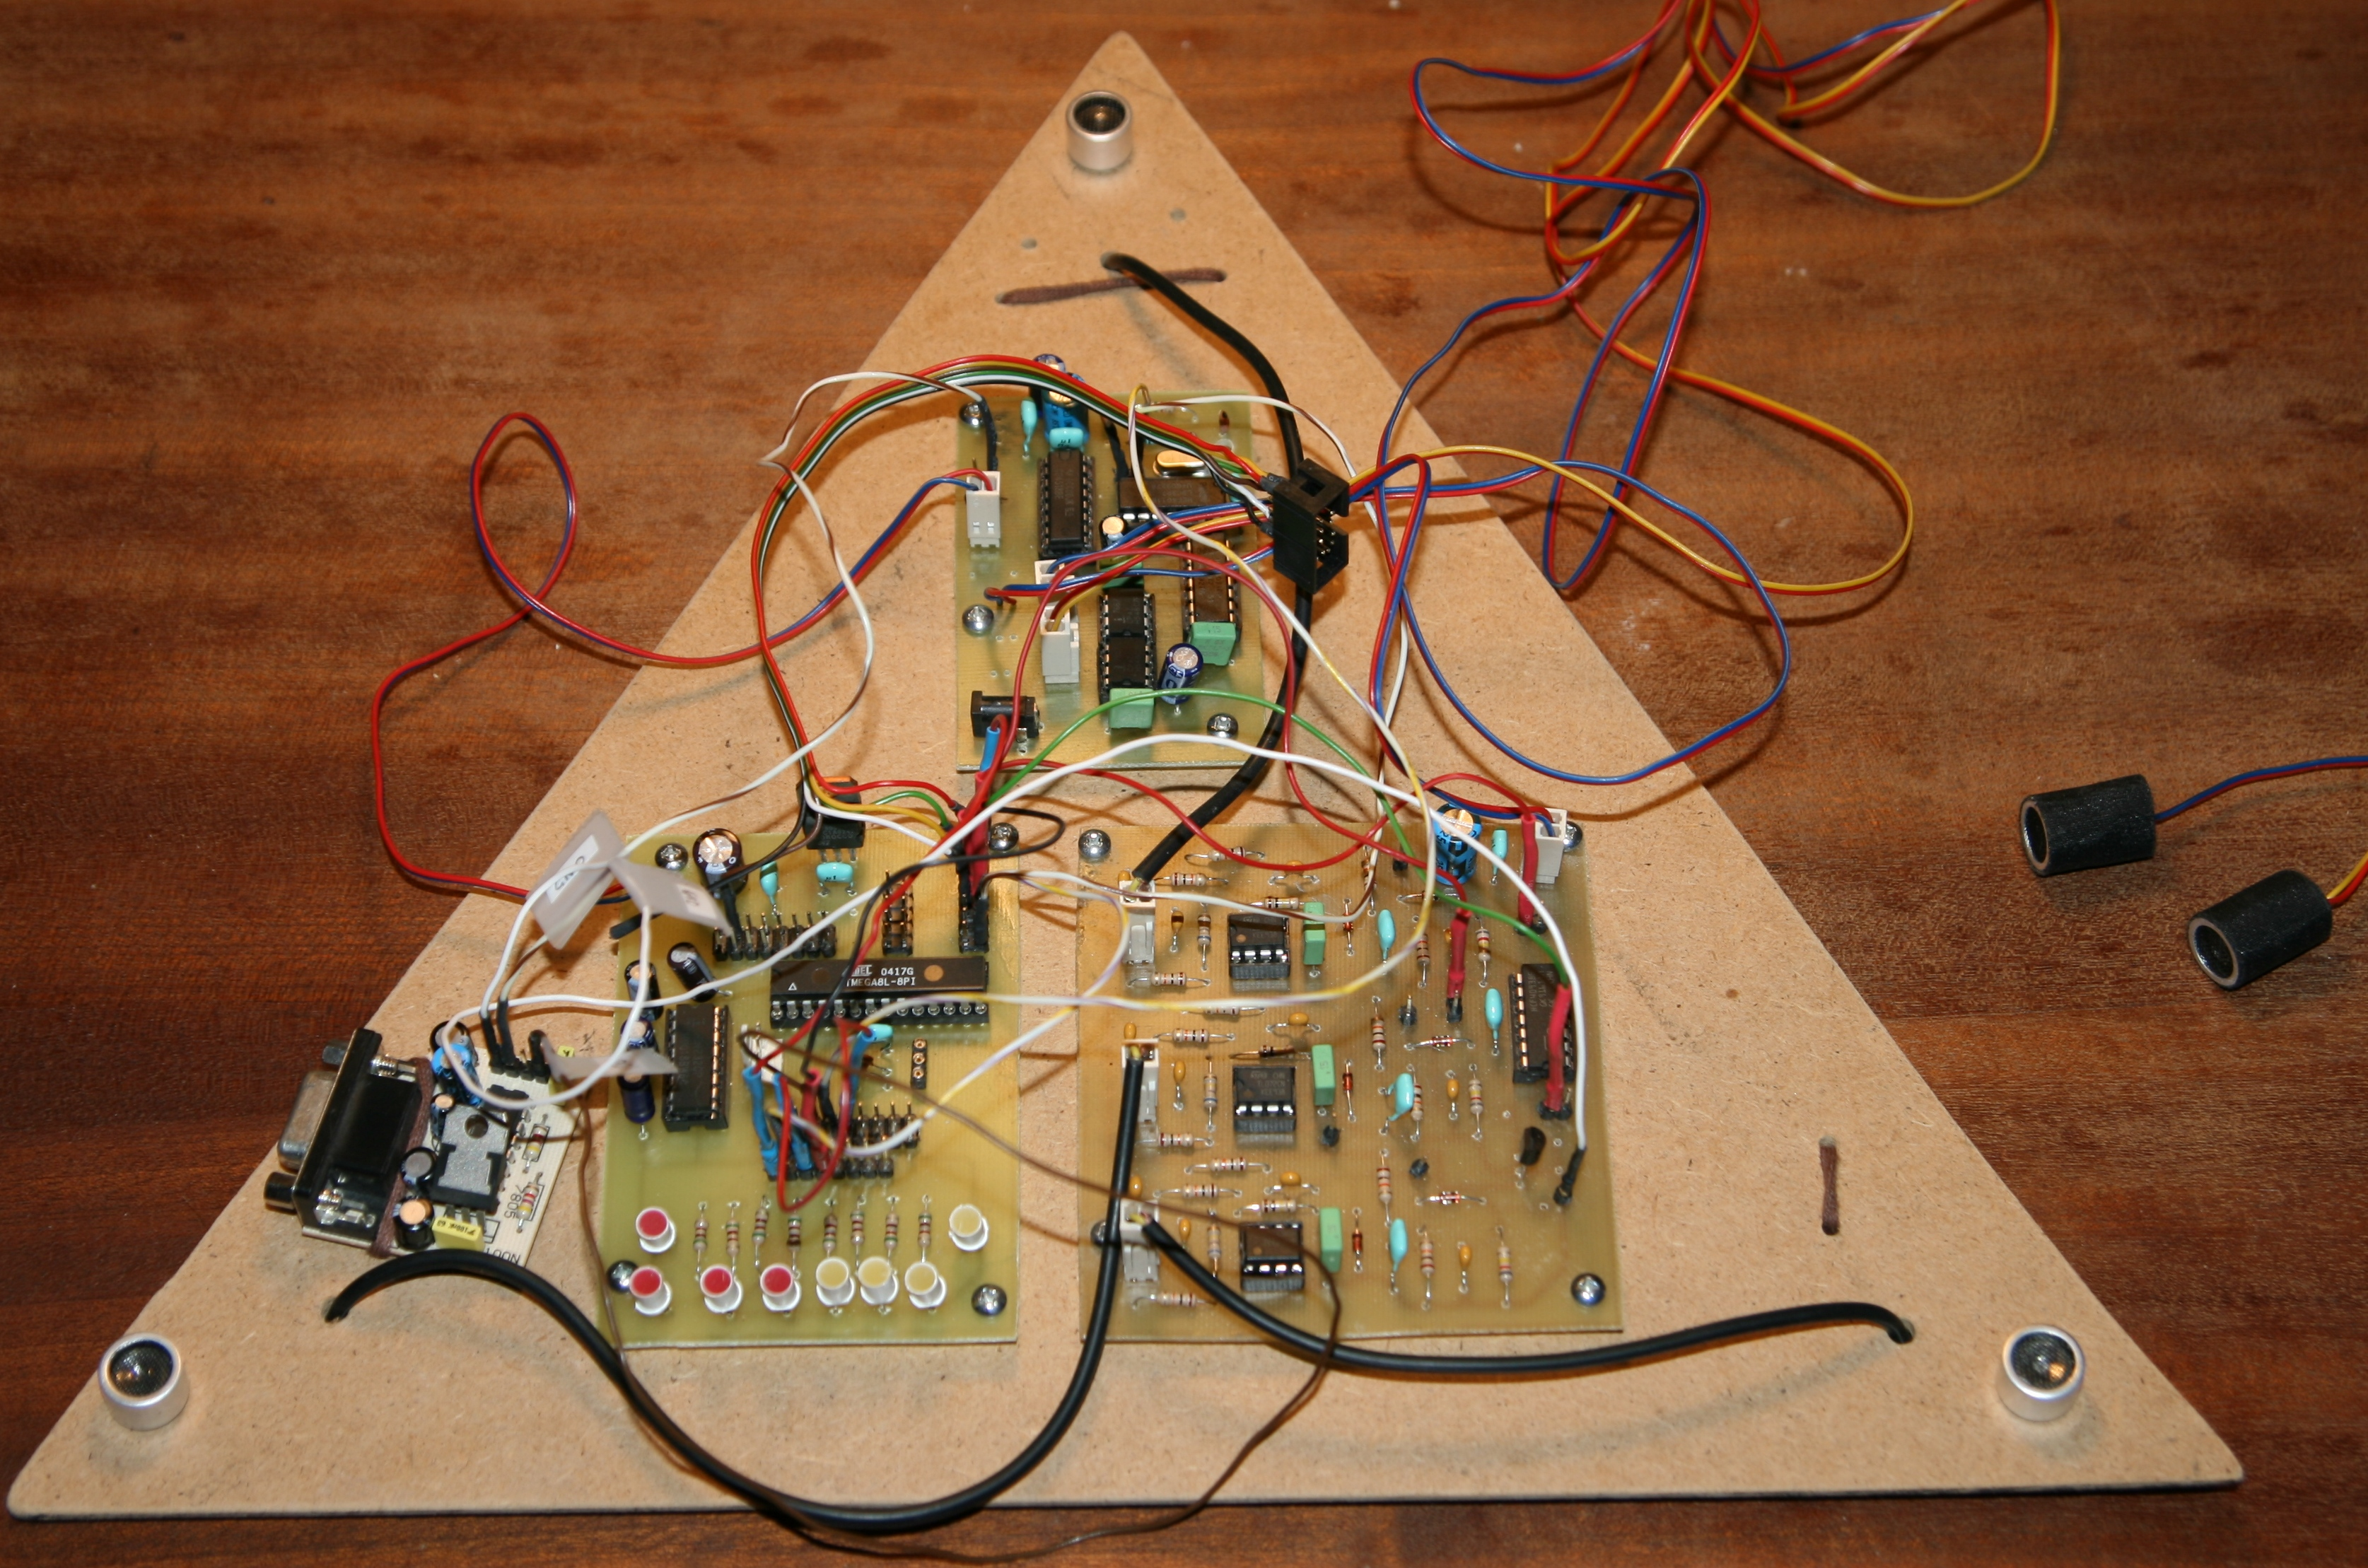
\includegraphics[width=\textwidth]{gfx/nietoperz.jpg}
  \caption{Nietoperz}
  \label{fig:nietoperz}
\end{sidewaysfigure}

Działanie mikrokontrolera sprowadza się do ciągłego, aktywnego prowadzenia pomiarów opóźnień czasów propagacji sygnału ultradźwiękowego pomiędzy \index{marker}markerami, a \index{odbiornik}odbiornikami. Pozyskane w ten sposób dane przekazywane są za pomocą specjalnie opracowanego \index{protokół}protokołu do komputera, gdzie następuje ich dalsza obróbka.

Uproszczony schemat układu prezentuje rysunek~\ref{fig:device_scheme}.

\begin{figure}
 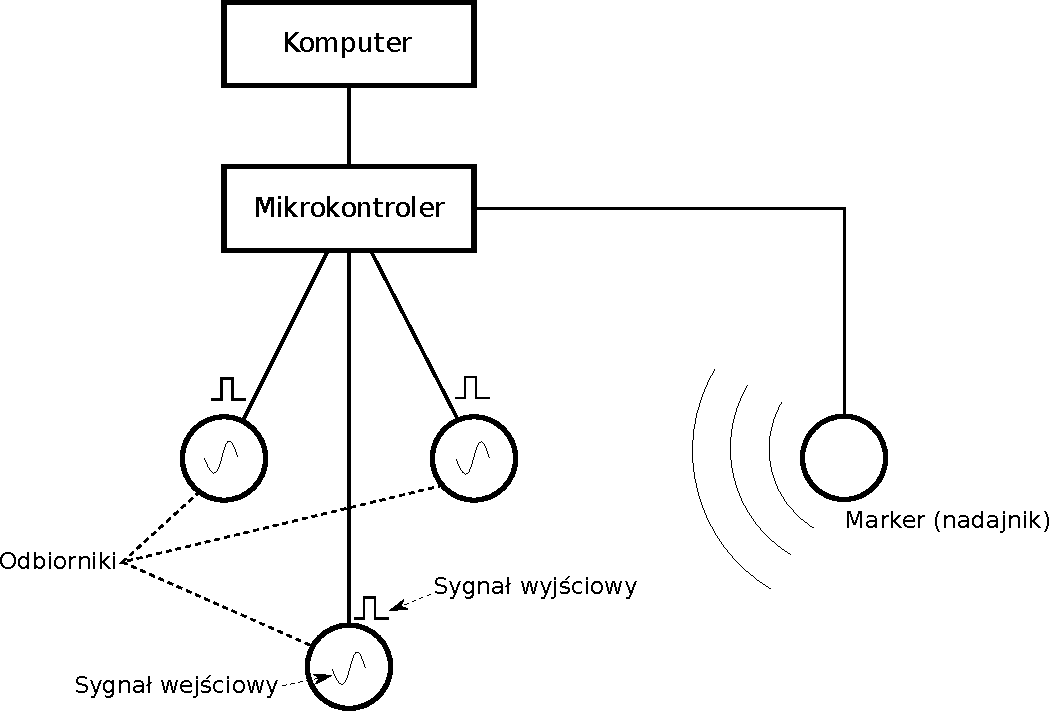
\includegraphics[width=\textwidth]{gfx/diagramy/schemat_blokowy_ukladu}
 \caption{Uproszczony schemat blokowy układu}
 \label{fig:device_scheme}
\end{figure}

Działanie systemu opiera się na założeniu, że dźwięk w powietrzu rozchodzi się ze stałą, znaną szybkością.\graffito{Założenie takie można przyjąć, gdyż odchylenia tej wartości spowodowane temperaturą i~wilgotnością powietrza są niewielkie i~nie wpływają znacząco na działanie systemu.}

Ponieważ szybkość ta jest stała, można łatwo wyznaczyć odległość, jaką musiał przebyć dźwięk, aby dotrzeć do odbiornika:
\begin{equation}
 x = v \cdot t
 \label{eq:sound_distance}
\end{equation}
gdzie:
%\graffito{dodać informację nt. kalibracji - zmiana protokołu na obsługę potwierdzeń, oczekiwanie mikrokontrolera na potwierdzenie, rozpoczynanie kalibracją, wymóg piramidki do kalibracji}
\begin{description}
 \item[$x$] \ppauza~odległość przebyta przez dźwięk,
 \item[$v$] \ppauza~szybkość dźwięku w powietrzu\graffito{Przyjęto prędkość dźwięku w powietrzu $v = 333\frac{\textrm{m}}{\textrm{s}}$.},
 \item[$t$] \ppauza~czas od wysłania sygnału do jego dotarcia do odbiornika. 
\end{description}

Dane, jakie przekazywane są do komputera w celu dalszej obróbki zawierają, poza sygnałami kontrolnymi \index{protokół}protokołu, również odczyty z~licznika dla każdego z~odbiorników, które zgodnie z wzorem \ref{eq:sound_distance} są proporcjonalne do odległości markera od tego odbiornika.

\paragraph{Przetwarzanie pozyskanych danych}
Ponieważ dane odczytane z mikrokontrolera mają postać ,,surową'', nie niosą one informacji, która jest możliwa do natychmiastowego wykorzystania w komputerze. Dopiero po przetworzeniu danych można pozyskać z nich wartościową informację. Przetwarzanie takie najczęściej wymagać będzie agregacji pewnej ilości danych oraz poddanie ich pewnemu procesowi obróbki. Proces ten stanowić może np.:
\begin{itemize}
 \item rozpoznawanie gestów,
 \item odtworzenie pozycji markera w trzech wymiarach,
 \item oczekiwanie na przemieszczenie markera do predefiniowanej pozycji.
\end{itemize}

\index{marker}
Jako demonstrację możliwości systemu pokażę, jak odtworzyć pozycję markera w trzech wymiarach, korzystając wyłącznie z~informacji o~względnym położeniu odbiorników oraz przekazywanych do komputera danych o czasie, w jakim sygnał z markera dotarł do każdego z tych odbiorników.

Aby wyznaczyć położenie markera w trójwymiarowej przestrzeni, mając do dyspozycji wymienione powyżej dane, można założyć, że odbiorniki są środkami sfer, a promieniem każdej z nich \ppauza odległość, jaką przebył dźwięk od markera do tego odbiornika. Punkt przecięcia się tych sfer będzie pozycją markera.

\begin{figure}
  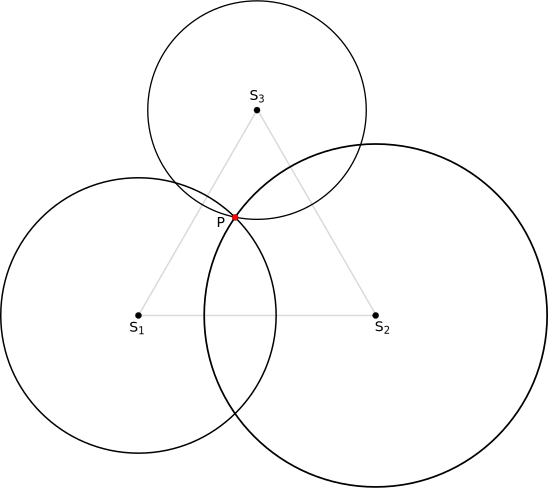
\includegraphics[width=\textwidth]{gfx/diagramy/schemat_przeciecia_sfer}
  \caption{Poglądowy schemat rozmieszczenia czujników}
  \label{fig:schema_spheres}
\end{figure}

Rysunek \ref{fig:schema_spheres}\graffito{W rysunku przyjęto widok ,,od przodu'', tzn. zachodzi $z = 0$ dla wszystkich elementów z~wyjątkiem punktu $P$.} prezentuje rozmieszczenie odbiorników na płycie testowej. Znajdują się one w punktach oznaczonych odpowiednio jako $S_1$, $S_2$ i $S_3$. Punkt $P$ to punkt przecięcia się sfer.

Ponieważ zastosowano tylko trzy \index{odbiornik}odbiorniki, będą one zawsze leżeć w jednej płaszczyźnie. Powoduje to, że dla każdego punktu $P$, będzie istniał punkt $P'$, który będzie odbiciem punktu $P$ względem płaszczyzne, w której zawarte są odbiorniki.
%\graffito{dodać notatkę w testach o możliwości wyeliminowania tego 'defektu' poprzez dodanie 4-tego odbiornika, niewspółpłaszczyznowego, jednak spowoduje to wzrost kosztów obliczeń}

Należy wziąć pod uwagę fakt, że zarówno marker jak i odbiorniki są urządzeniami ,,kierunkowymi'', umieszczonymi w tulejach, które powodują, że sygnał nie jest wysyłany dookólnie, lecz w pewnym \ppauza z grubsza określonym \ppauza kierunku, zaś amplituda sygnału odbieranego będzie większa, jeśli będzie on wpadał prosto w tuleję\graffito{Sygnał dochodzący z~boku może być zbyt słaby, aby został zarejestrowany.}, przez co szansa uznania go za poprawny jest znacznie większa.

Ta cecha układu została wykorzystana poprzez przeznaczenie układu do noszenia na tułowiu \ppauza łatwo zauważyć, że użytkownikowi ciężko byłoby przesunąć \index{marker}marker zbyt daleko do tyłu, gdyż ograniczałyby go stawy. 

Wykorzystując fakt, że człowiek trzyma ręce w większości przypadków przed sobą, szczególnie jeśli zamierza coś nimi robić, można spokojnie odrzucić jeden z punktów \ppauza ten który znajduje się ,,z tyłu''.

\paragraph{Pomiar czasu pomiędzy wysłaniem, a odebraniem sygnału}
\label{sec:uc_algorithm}
Z powodu tego, iż dostępne markery nadają tylko na jednej, ustalonej częstotliowści konieczne okazało się wykonanie procesu pomiarowego z podziałem czasu. Oznacza to, iż w jednej chwili czasu nadaje tylko i wyłącznie jeden marker, prowadzony jest więc pomiar tylko dla jednego kanału, a informacja o jego parametrach jest wstępnie przetwarzana, zapisywana i przesyłana do komputera. Odbywa się to w~następujący sposób:
\begin{enumerate}
 \item \index{prescaler}prescaler\graffito{Opis prescalera znajduje się poniżej.} urządzenia jest resetowany,\label{enum:prescaler}
 \item uruchamiany jest wewnętrzny licznik urządzenia,
 \item wysyłany jest sygnał, który aktywuje jeden z markerów, powoduje to rozpoczęcie nadawania sygnału przez ten marker,
 \item następuje aktywne oczekiwanie na ,,wzbudzenie''\graffito{Wzbudzenie pinu to przejście linii z~sygnału niskiego do stanu wysokiego.} pinów wszystkich odbiorników, a czas wzbudzenia każdego z pinów (różnica czasu pomiędzy rozpoczęciem nadawania i odebrania sygnału z~danego odbiornika) jest zapamiętywany,
 \item zatrzymywany jest wewnętrzny timer urządzenia,
 \item dane o odstępach czasowych przekazywane są do komputera,
 \item następuje uśpienie układu, które pozwala na zaniknięcie sygnałów ultradźwiękowych,
 \item cała operacja powtarzana jest dla następnego markera.
\end{enumerate}
Algorytm ten obrazuje diagram przedstawiony na rysunku \ref{fig:firmware_sequence_diagram}.

\begin{figure}
 % fugly hack
 \hspace{-7em}
 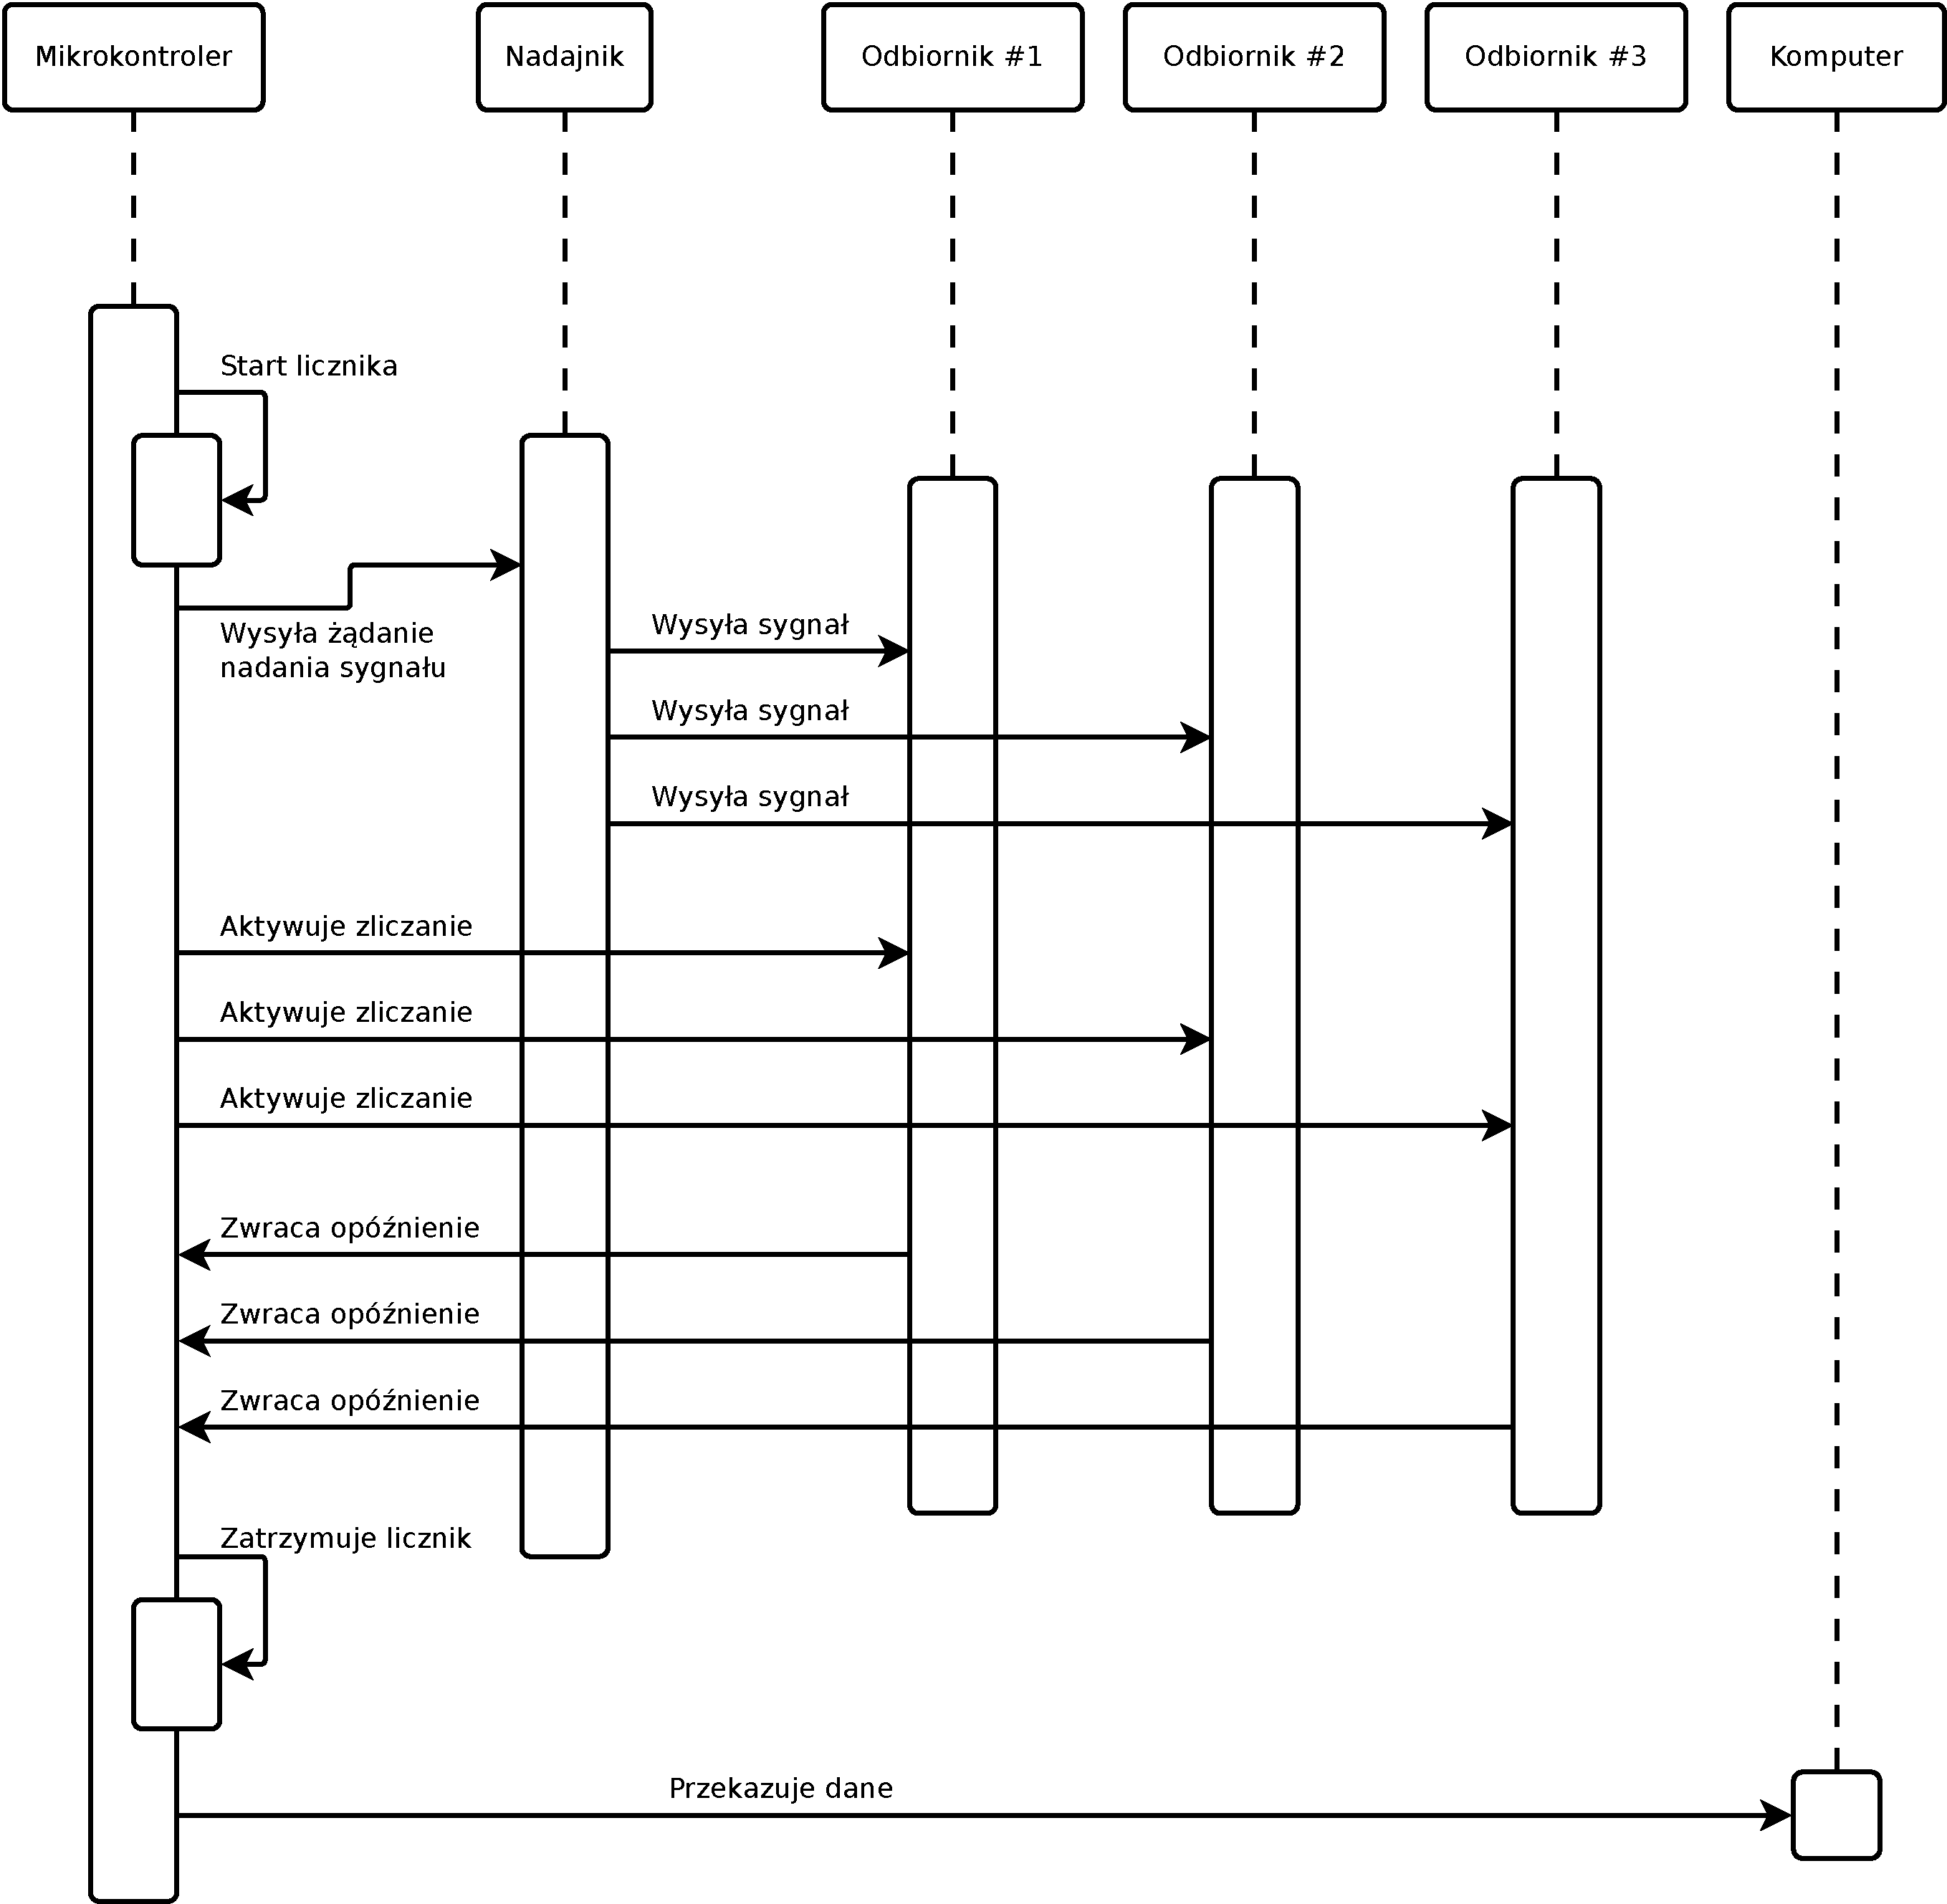
\includegraphics[width=52em]{gfx/diagramy/diagram_sekwencji_sprzetu.pdf}
 \caption{Diagram sekwencji oprogramowania mikrokontrolera}
 \label{fig:firmware_sequence_diagram}
\end{figure}

W mikrokontroler wbudowany jest \index{prescaler}\textsl{prescaler}, czyli dzielnik częstotliwości, o programowanym stopniu podziału. Jego działanie polega na zliczaniu taktów zegara; gdy wewnętrzny licznik prescalera osiągnie zaprogramowaną wcześniej wartość, wyzwalane jest przerwanie timera oraz następuje przepełnienie licznika, w związku z czym zliczana wartość ,,przekręca się'' i liczenie rozpoczyna się ponownie od zera.
\label{sec:prescaler}

Wyzerowanie prescalera przed rozpoczęciem pomiaru ma istotny wpływ na dokładność danych. Załóżmy na chwilę, że prescaler nie jest resetowany. Ponieważ nie ma możliwości\graffito{Nawet gdyby możliwość odczytania tej wartości istniała, działanie to wprowadzałoby niepożądane opóźnienia.} sprawdzenia aktualnego stanu licznika prescalera, nie możemy stwierdzić ile czasu upłynęło od ostatniego wyzwolenia przerwania timera. Bez znajomości tej wartości nie jest możliwe stwierdzenie, kiedy, licząc od zapisania bitów uruchamiających moduł timera, nastąpi wywołanie przerwania timera. Powyższe fakty powodują, że dla każdego z pomiarów będzie istniało pewne \emph{nieznane} opóźnienie rozpoczęcia naliczania interwału czasowego, co bezpośrednio przekłada się na dokładność pozyskanych danych.

Resetowanie prescalera zawsze w tym samym miejscu zapewnia, że każdy pomiar rozpocznie się z dokładnie takim samym opóżnieniem.

\paragraph{Trilateracja}
\label{par:trilateration}
\index{trilateracja}
Metoda wyznaczenia trójwymiarowej pozycji znając odległości od trzech punktów o znanych współrzędnych nazywana jest \textit{trilateracją}.%\graffito{dodać info skąd to wiadomo}

Problem wyznaczenia położenia markera można uprościć, przyjmując określony układ współrzędnych, w którym jeden z odbiorników znajduje się w początku układu współrzędnych, drugi na osi $x$, a trzeci pozostaje ,,swobodny''\graffito{Współrzędna $z$ dla wszystkich odbiorników równa jest~$0$.}. Rozmieszczenie takie zaprezentowano na rysunku \ref{fig:schema_coordinates}, odbiorniki mają współrzędne odpowiednio:
\begin{center}
 $S_1 (0, 0)$

 $S_2 (a, 0)$

 $S_3 (b, c)$
\end{center}

\begin{figure}
  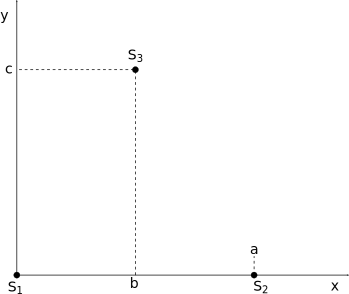
\includegraphics[width=\textwidth]{gfx/diagramy/schemat_uklad_wspolrzednych_clipped}
  \caption{Układ współrzędnych wykorzystany do określenia pozycji odbiorników}
  \label{fig:schema_coordinates}
\end{figure}

Równanie sfery ze środkiem w punkcie o współrzędnych $(x_0, y_0, z_0)$ i promieniu $r$ przyjmuje postać:
\begin{equation}
 r = \sqrt{(x - x_0)^2 + (y - y_0)^2 + (z - z_0)^2}
 \label{eq:sphere}
\end{equation}

Podstawiając do równania \ref{eq:sphere} współrzędne punktów $S_1$, $S_2$ i $S_3$ otrzymujemy następujący układ równań:
\begin{equation}
 \begin{cases}
  r_1 = \sqrt{x^2 + y^2 + z^2} \\
  r_2 = \sqrt{(x - a)^2 + y^2 + z^2} \\
  r_3 = \sqrt{(x - b)^2 + (y - c)^2 + z^2}
 \end{cases}
 \label{eq:sphere_system_1}
\end{equation}
gdzie $r_1$, $r_2$ i $r_3$ to odpowiednio odległości \index{marker}markera od każdego z~odbiorników\index{odbiornik} \textsmaller{\#1}, \textsmaller{\#2} i \textsmaller{\#3}, a zarazem promienie sfer, których punktu przecięcia poszukujemy.

Wartości $r_1$, $r_2$ i $r_3$ obliczamy na podstawie danych $t_1$, $t_2$ i $t_3$, czyli odstępie czasu, jaki dzieli rozpoczęcie nadawania przez marker od odebrania tego sygnału przez mikrokontroler. Wykorzystując równanie \ref{eq:sound_distance} otrzymujemy:
\begin{eqnarray}
  r_n = 333\frac{\textrm{m}}{\textrm{s}} \cdot t_n & \textrm{dla } n \in \{1, 2, 3\}
\end{eqnarray}


W celu uproszczenia następnych obliczeń przyjmijmy poniższą postać równania \ref{eq:sphere_system_1}:
\begin{equation}
 \begin{cases}
  r_1^2 = x^2 + y^2 + z^2 \\
  r_2^2 = (x - a)^2 + y^2 + z^2 \\
  r_3^2 = (x - b)^2 + (y - c)^2 + z^2
 \end{cases}
 \label{eq:sphere_system_2}
\end{equation}

Rozwińmy najpierw drugie równanie z układu \ref{eq:sphere_system_2}:
\begin{equation}
 r_2^2 = (x - a)^2 + y^2 + z^2 = x^2 - 2xa + a^2 + y^2 + z^2
\end{equation}

Następnie odejmijmy je od równania pierwszego z systemu \ref{eq:sphere_system_2}:
\begin{equation}
 r_1^2 - r_2^2 = x^2 + y^2 + z^2 - (x^2 - 2xa + a^2 + y^2 + z^2) = 2xa - a^2
 \label{eq:determine_x_1}
\end{equation}

Z równania \ref{eq:determine_x_1} można łatwo wyznaczyć $x$:
\begin{eqnarray}
 r_1^2 - r_2^2 = 2xa - a^2 & | & + a^2\\
 r_1^2 - r_2^2 + a^2 = 2xa & | & \colon 2a\\
 x = \frac{r_1^2 - r_2^2 + a^2}{2a} \label{eq:determine_x_2}
\end{eqnarray}

Podstawiając $x$ z równania \ref{eq:determine_x_2} do pierwszego równania układu \ref{eq:sphere_system_2} dowiemy się, które punkty są wspólne dla sfer mających środki w,~odpowiednio, $S_1$ i $S_2$:

\begin{eqnarray}
 r_1^2 & = & x^2 + y^2 + z^2 \\
       & = &\left(\frac{r_1^2 - r_2^2 + a^2}{2a}\right)^2 + y^2 + z^2 \nonumber \\
 y^2 + z^2 & = & r_1^2 - \left(\frac{r_1^2 - r_2^2 + a^2}{2a}\right)^2 \label{eq:intersection_circle}
\end{eqnarray}

W równaniu \ref{eq:intersection_circle} prawa strona jest stała, widać więc, że jest to równanie okręgu.

Rozwińmy teraz równanie trzeciej sfery:
\begin{eqnarray}
 r^2_3 & = & (x - b)^2 + (y - c)^2 + z^2 \label{eq:third_sphere} \\
       & = & x^2 - 2bx + b^2 + y^2 - 2cy + c^2 + z^2 \nonumber
\end{eqnarray}

Podstawiając równanie pierwszej sfery przekształcone do postaci
\begin{equation*}
 y^2 + z^2 = r_1^2 - x^2
\end{equation*}
do wzoru \ref{eq:third_sphere} otrzymujemy:
\begin{eqnarray}
r_3^2 & = & x^2 - 2bx + b^2 - 2cy + c^2 + r_1^2 - x^2 \label{eq:third_sphere_substituted} \\
      & = & -2bx + b^2 - 2cy + c^2 + r_1^2 \nonumber
\end{eqnarray}

Na podstawie równania \ref{eq:third_sphere_substituted} można wyznaczyć $y$:
\begin{eqnarray}
 r_3^2 = -2bx + b^2 - 2cy + c^2 + r_1^2 & | & +2cy - r_3^2 \\
 2cy   = -2bx + b^2 + c^2 + r_1^2 - r_3^2 & | & \colon 2c \\
 y     = \frac{-2bx + b^2 + c^2 + r_1^2 - r_3^2}{2c} & & \label{determine_y}
\end{eqnarray}

Ponieważ $x$ jest stałe, jak pokazuje równanie \ref{eq:determine_x_2}, to prawa strona równania \ref{determine_y} również będzie stała.

Do wyznaczenia pozostało jeszcze jedynie $z$. Aby policzyć jego wartość, weźmy wzór pierwszej sfery z układu \ref{eq:sphere_system_1}, stąd $z$ będzie wynosić:
\begin{equation}
 z = \pm\sqrt{r_1^2 - x^2 - y^2}
\end{equation}

Jak jednak pamiętamy z opisu, jeden z tych punktów, ,,tylny'' odrzucamy, w związku z czym $z$ ostatecznie przyjmuje postać:
\begin{equation}
 z = \sqrt{r_1^2 - x^2 - y^2}
\end{equation}

Reasumując, jeśli przyjąć rozmieszczenie \index{odbiornik}odbiorników takie jak na rysunku~\ref{fig:schema_coordinates}, punkt przecięcia się sfer\graffito{Dla uproszczenia przyjmujemy, że punkt taki zawsze istnieje, co w~skonstruowanym systemie jest prawdziwe.} będzie miał następujące współrzędne:
%\graffito{dodać info o lokalności układu i konieczności jego odtworzenia}
\begin{eqnarray}
 x & = & \frac{r_1^2 - r_2^2 + a^2}{2a} \label{eq:trilateration_final_x}\\
 y & = & \frac{-2bx + b^2 + c^2 + r_1^2 - r_3^2}{2c} \label{eq:trilateration_final_y}\\
   & = & \frac{-b\frac{r_1^2 - r_2^2 + a^2}{a} + b^2 + c^2 + r_1^2 - r_3^2}{2c} \nonumber \\
 z & = & \sqrt{r_1^2 - x^2 - y^2} \label{eq:trilateration_final_z}\\
   & = & \sqrt{r_1^2 - \left(\frac{r_1^2 - r_2^2 + a^2}{2a}\right)^2 - \left(\frac{b\frac{r_1^2 - r_2^2 + a^2}{-a} + b^2 + c^2 + r_1^2 - r_3^2}{2c}\right)^2} \nonumber
\end{eqnarray}

Jako ciekawostkę warto dodać informację, że system \textsc{GPS} korzysta z~bardzo podobnej metody (chociaż jej implementacja jest zupełnie inna) \citep{MioGps}.
